\section{Case Study}

A single test case was simulated to visually determine the brightness of the Cherenkov peak and any interesting features. The test shower had an energy of \SI{e19}{eV}, an impact parameter of \SI{10}{km}, and an axis pointing slightly rightward and away from the detector. Figure \ref{fig:typical_map} shows the view from the detector after the addition of noise. The sky-ground boundary is visible as a drop in the level of background noise at $y = 120$. Figure \ref{fig:typical_graph} shows the time profile before the addition of noise. In the first portion, the shower moves downward and produces fluorescence photons. At about \SI{0.128e-3}{s}, there is a sharp peak from the reflected Cherenkov radiation. The tails of this peak are caused by Cherenkov rays with large deviations from the shower axis. The brightness of the Cherenkov peak prompts a hybrid reconstruction. Before reconstruction, noise filtration is performed. For a well-behaved shower like this, the core of the fluorescence track remains intact, and only 1-2 photoelectron signals near the fringes are removed. Figure \ref{fig:typical_denoise_map} shows the spatial profile after this process. The actual impact parameter and angle are \SI{10}{km} and \ang{72.5}. The monocular reconstruction gives \SI{9.75}{km} and \ang{71.3}, whereas the Cherenkov reconstruction gives \SI{10.6}{km} and \ang{75.2}.

\begin{figure}[!ht]
    \label{fig:typical_map}
    \centering
    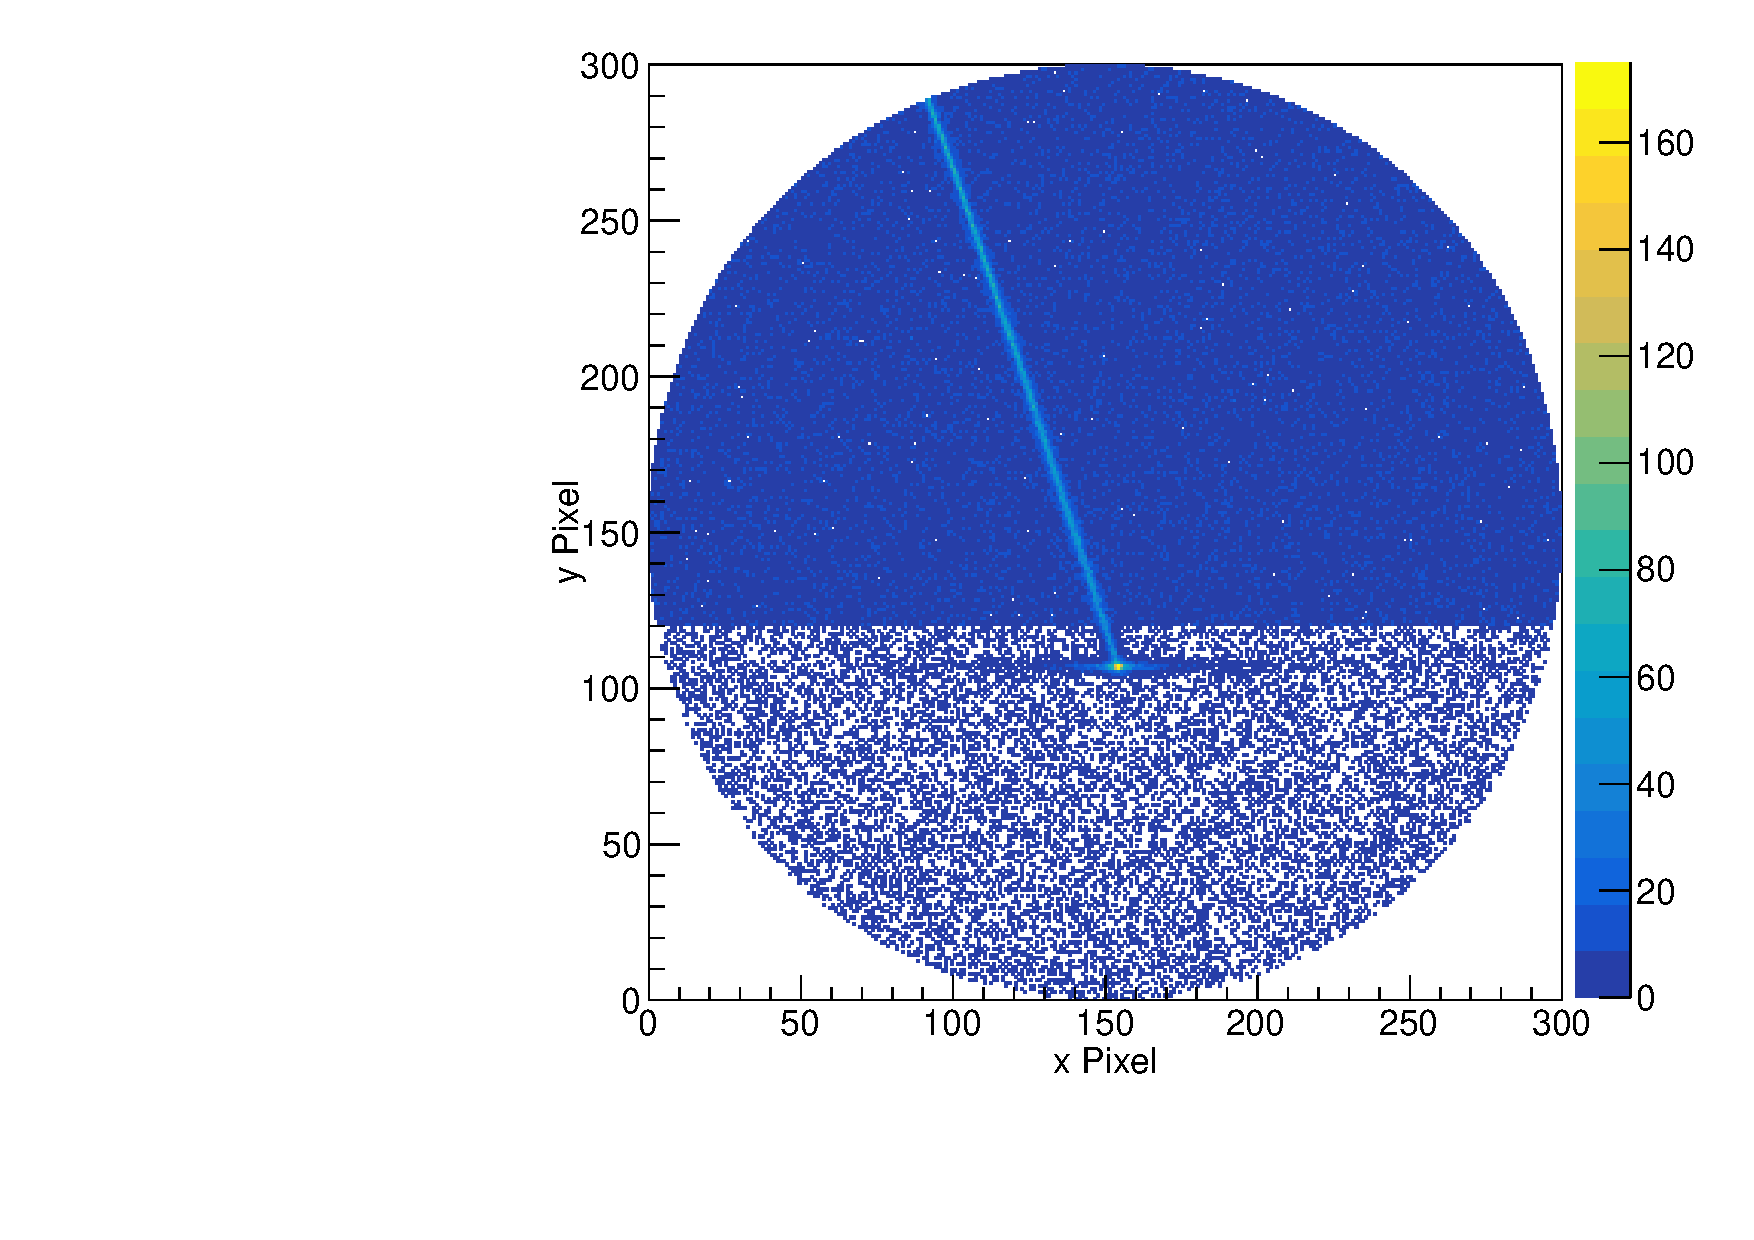
\includegraphics[width=\textwidth]{TypicalShowerMap}
    \caption{A spatial view of a typical shower track with noise added. This event has energy \SI{e19}{eV}, angle \ang{72.5}, and impact parameter \SI{10}{km}.  The ground impact is visible near pixel (150, 100).}
\end{figure}

\begin{figure}[!ht]
    \label{fig:typical_graph}
    \centering
    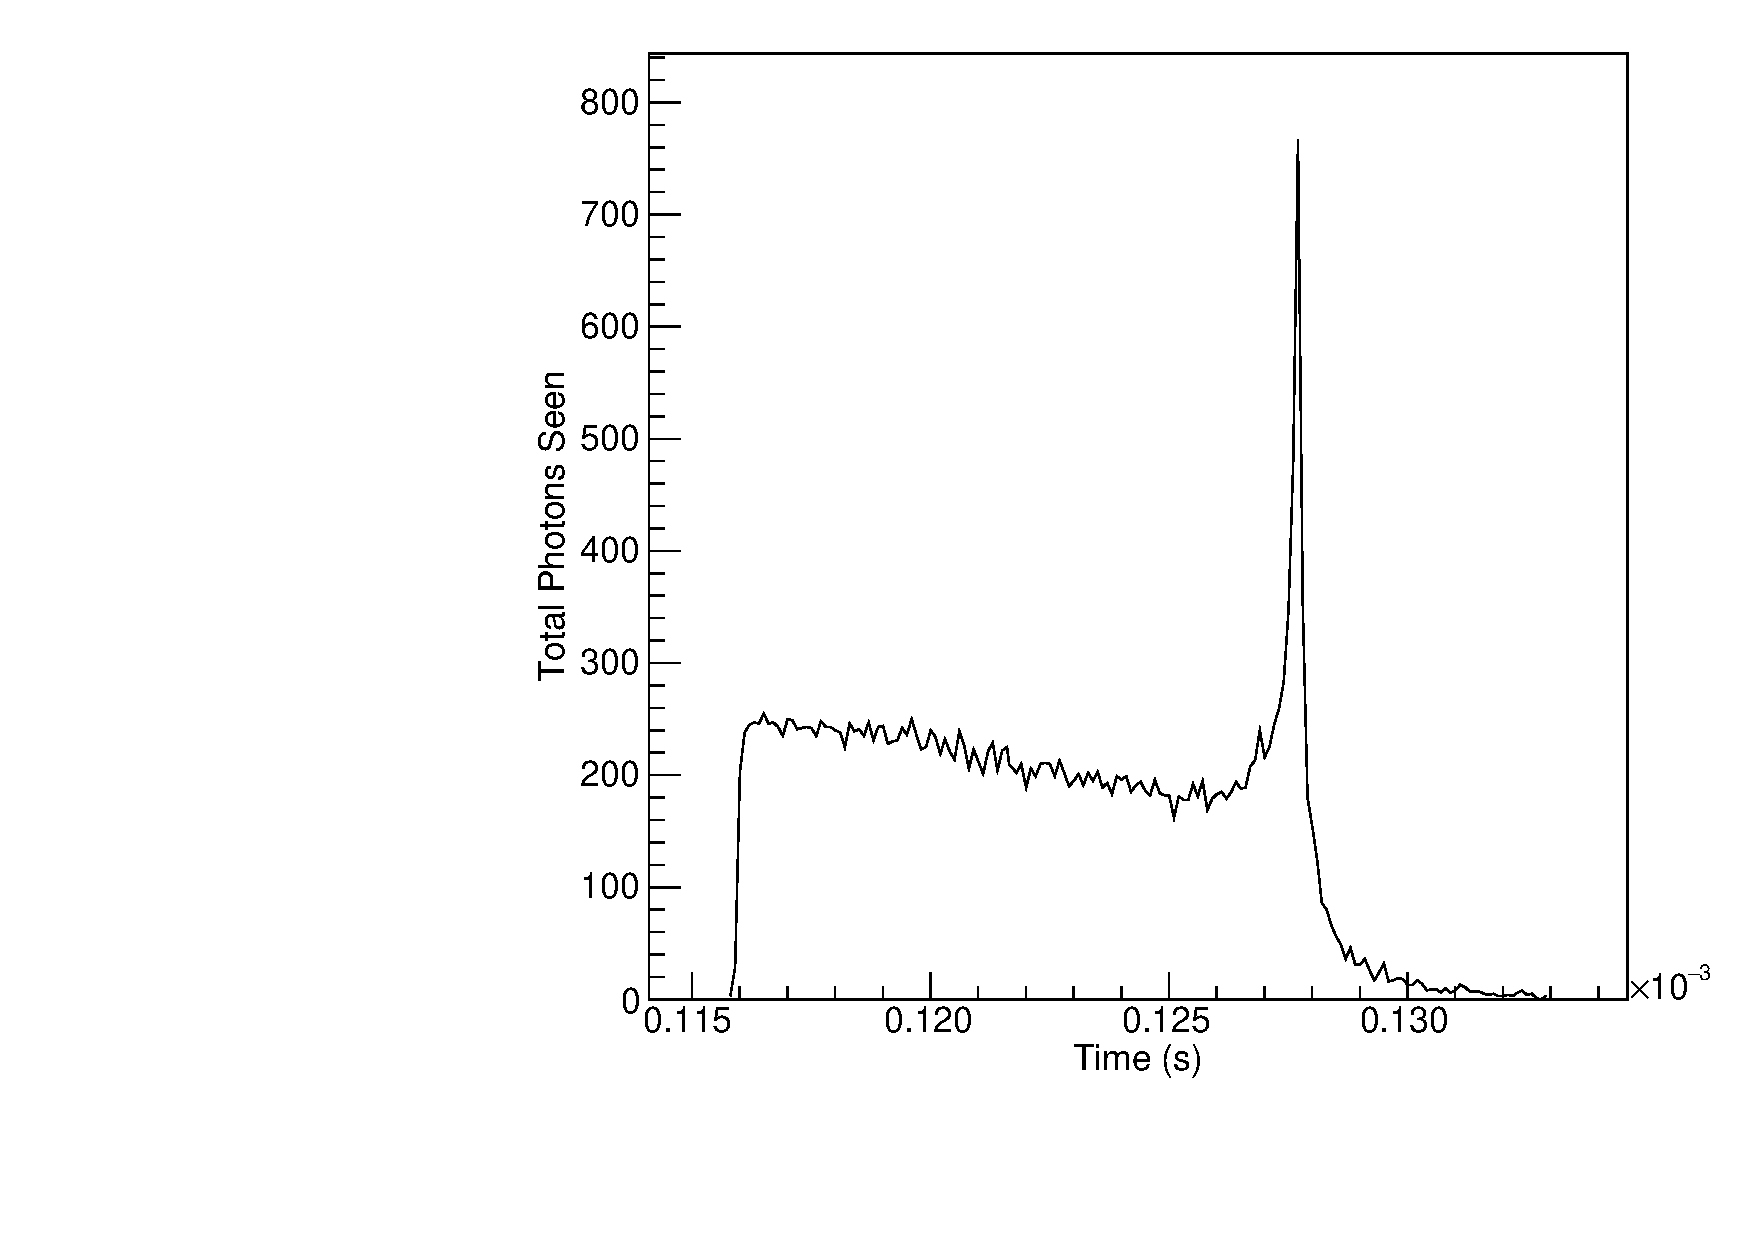
\includegraphics[width=\textwidth]{TypicalShowerGraph}
    \caption{Signal versus time for the event shown in Figure \ref{fig:typical_map}. The Cherenkov peak is visible near \SI{0.128e-3}{s}. The fluorescence portion decays because of the shower direction and because the Gaisser-Hillas maximum has been passed.}
\end{figure}

\begin{figure}[!ht]
    \label{fig:typical_denoise_map}
    \centering
    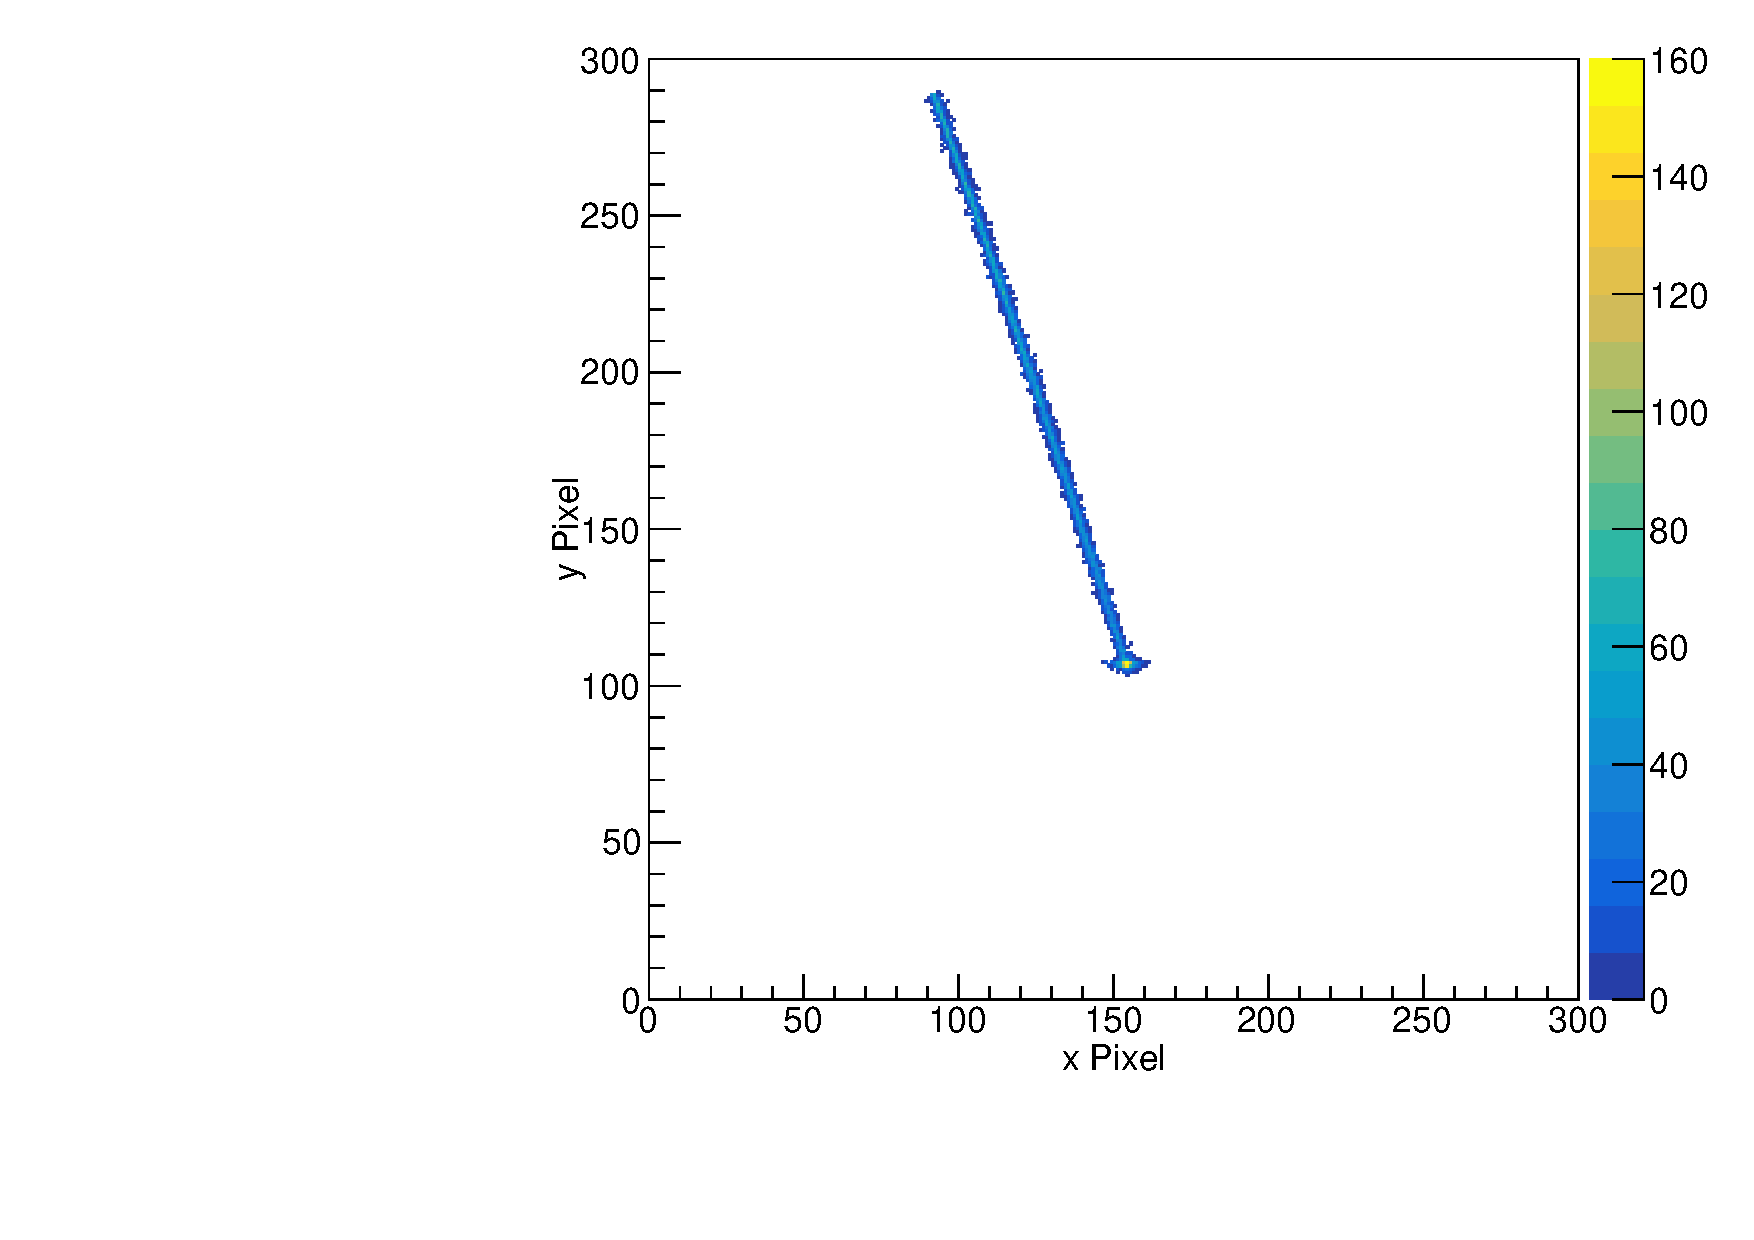
\includegraphics[width=\textwidth]{TypicalDenoiseMap}
    \caption{The shower track from Figure \ref{fig:typical_map} after the removal of noise. The fluorescence core and impact point are still visible, but their fringes have contracted.}
\end{figure}

\section{Monte Carlo} \label{sec:mc_results}

The initial Monte Carlo run simulated \num{12000} triggered showers with a \SI{200}{m} high detector. Impact parameters were distributed between \num{3} and \SI{40}{km}, and energies were chosen from an $E^{-1}$ distribution between \num{e17} and \SI{e21}{eV}. About \num{8300} of the \num{12000} showers met the requirements for Cherenkov reconstruction. In analyzing these events, we examine both error in the impact parameter and error in the angle. However, as Figure \ref{fig:correlation} shows, there is a strong correlation between the two. Because of this, only trends in impact parameter error were examined.

\begin{figure}[p]
    \label{fig:correlation}
    \centering
    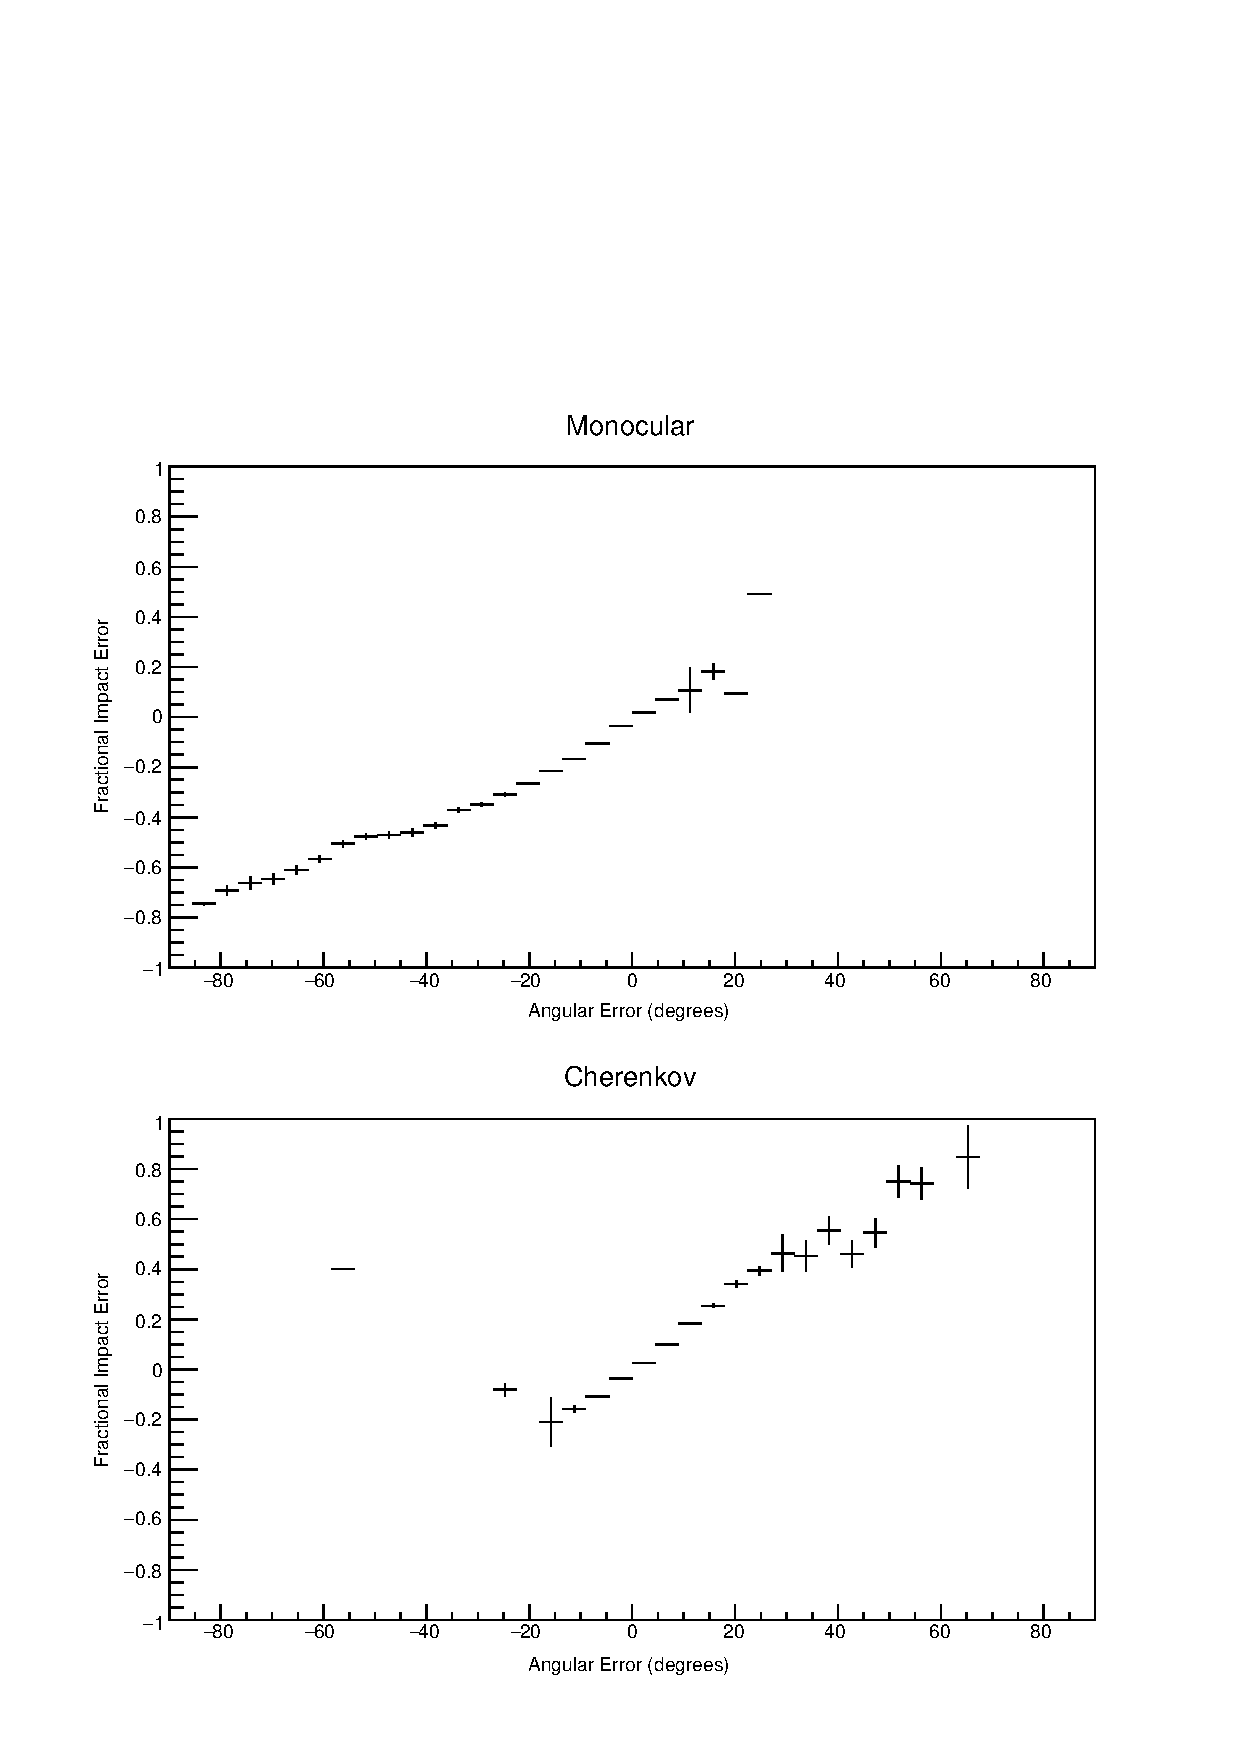
\includegraphics[width=\textwidth]{Correlation}
    \caption{The correlation between error in impact parameter and error in angle, eliminating the need for an independent analysis of each.}
\end{figure}

Figures \ref{fig:error_vs_impact} and \ref{fig:error_vs_angle} illustrate the relationships between fractional impact parameter error and both angle and impact parameter. The Cherenkov reconstruction does well when the impact parameter is less than \SI{25}{km}, although the monocular reconstruction also does fairly well in this range. As expected, the monocular reconstruction does poorly when the shower angle is large. At large angles, the track is compressed in the detector's field of view, and some of the angle versus time information is lost. Somewhat surprisingly, the Cherenkov reconstruction does poorly when the shower angle is small. Below \ang{40}, the average errors exceed the bounds of the graph, and can be on the order of 200-300 percent. These errors are rooted in the relative brightness of the fluorescence track and the Cherenkov reflection point. As the shower angle shrinks, the reflection point gets more distant. While both the fluorescence track and reflection point get dimmer via a standard $1/r^2$ dropoff, the Cherenkov reflection also gets dimmer as $\sin{\alpha}$ due to the nature of Lambertian reflectance ($\alpha$ is the angle of the reflection point from the horizon). This additional $\sin{\alpha}$ factor causes the reflection point to get dimmer more quickly than the fluorescence track. At a certain distance, the reflectance point is overtaken in brightness by the fluorescence track. When this occurs, the ground point algorithm incorrectly chooses a point on the fluorescence track, often adjacent to the horizon. This results in an extreme overestimate of the ground distance and, by extension, of the impact parameter.

\begin{figure}[p]
    \label{fig:error_vs_impact}
    \centering
    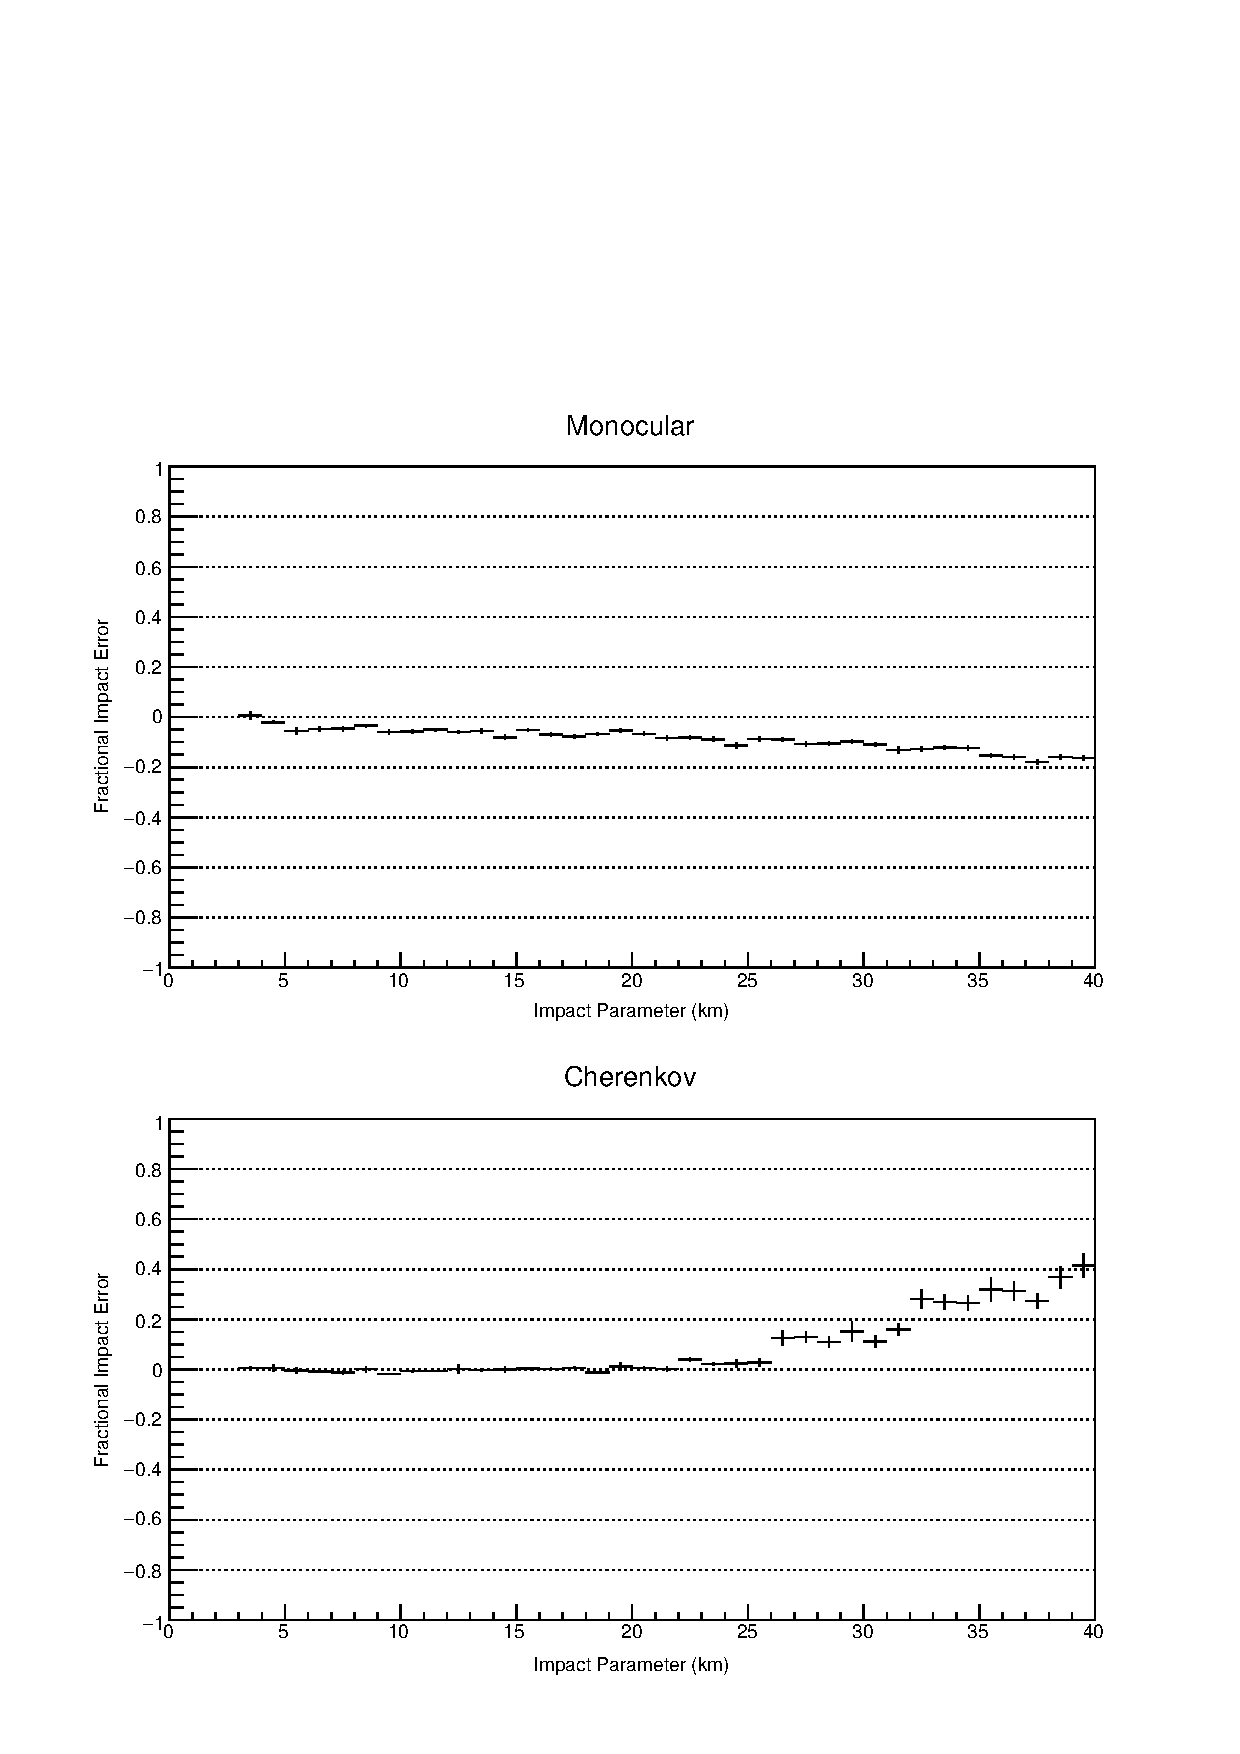
\includegraphics[width=\textwidth]{InitialVersusImpact}
    \caption{Results from the initial run with a \SI{200}{m} high detector. Shows the relationship between reconstruction error and impact parameter, for both monocular and Cherenkov methods.}
\end{figure}

\begin{figure}[p]
    \label{fig:error_vs_angle}
    \centering
    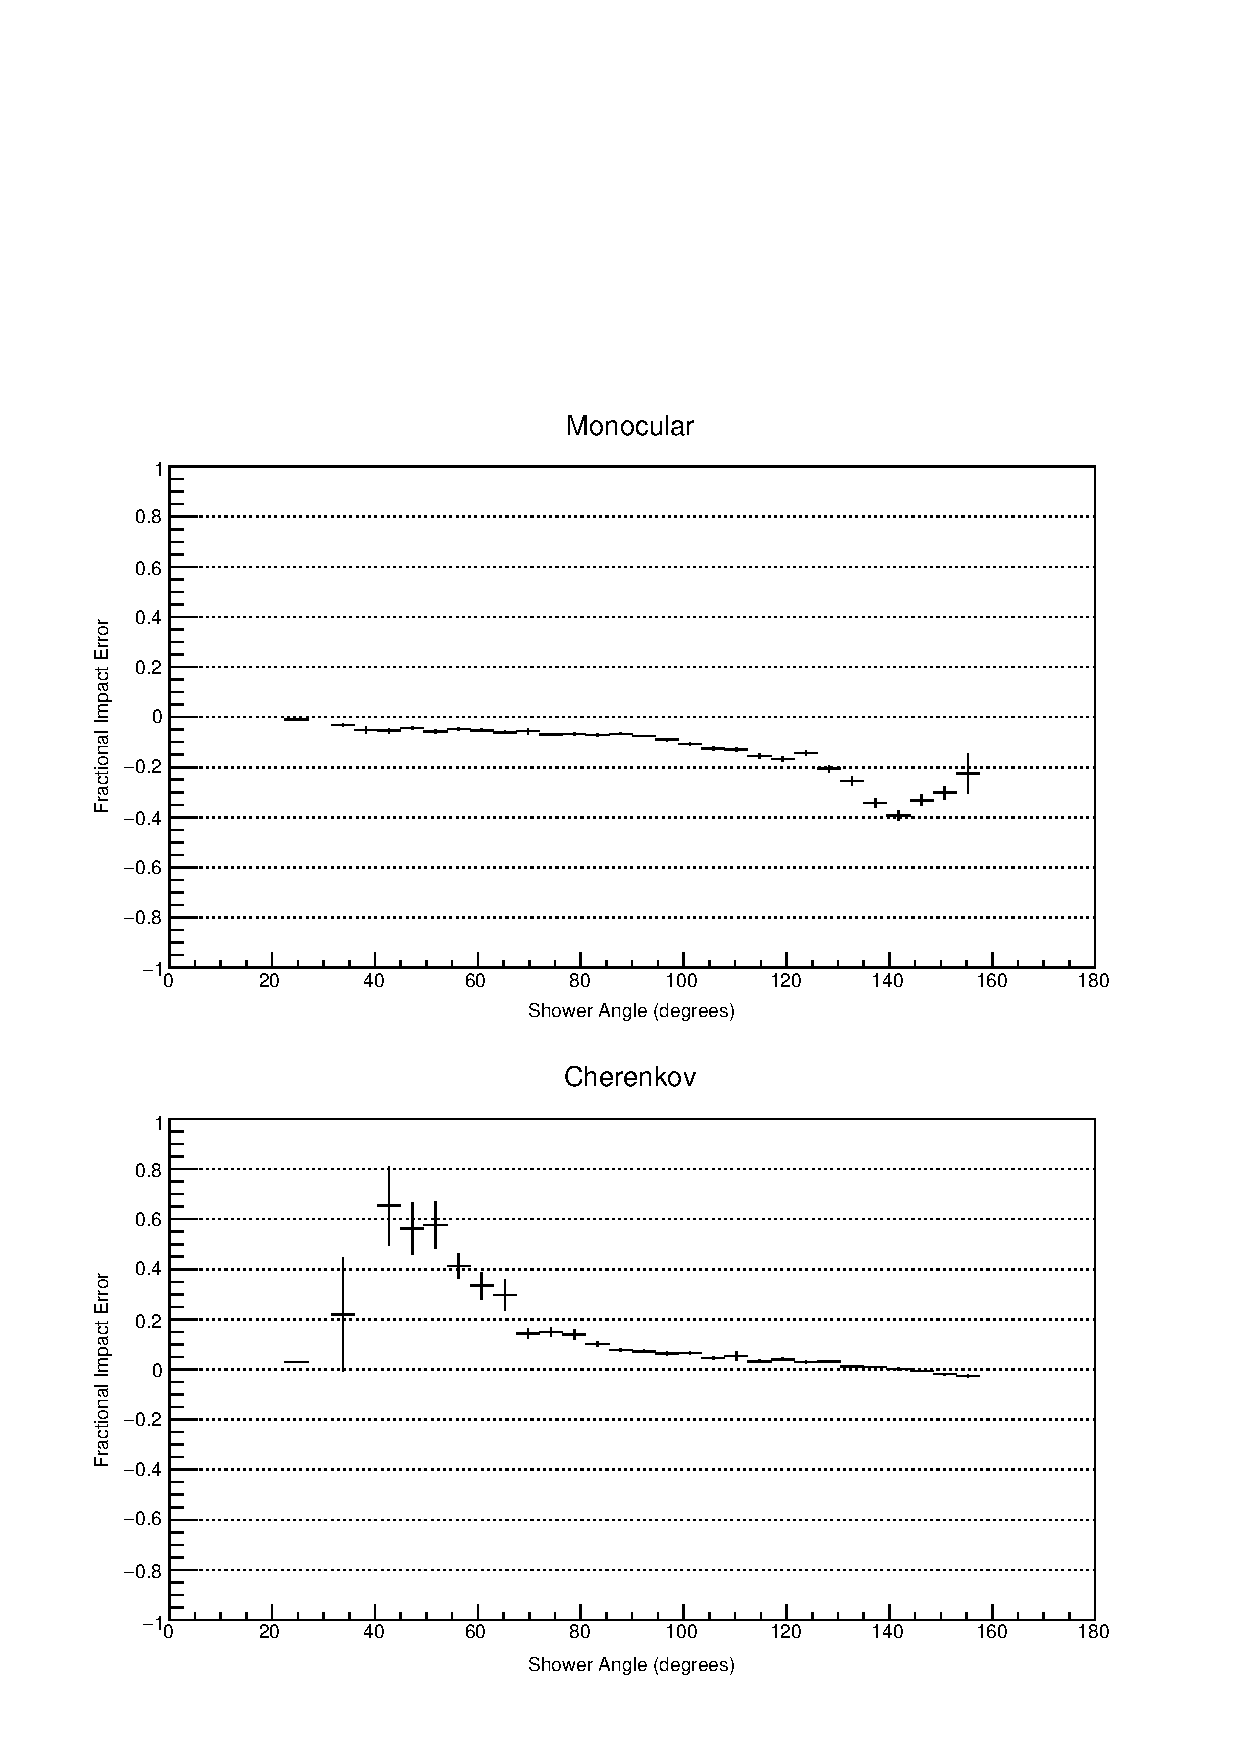
\includegraphics[width=\textwidth]{InitialVersusPsi}
    \caption{Results from the initial run with a \SI{200}{m} high detector. Shows the relationship between reconstruction error and shower angle, for both monocular and Cherenkov methods. Some of the average errors for small angle Cherenkov reconstructions exceed the bounds of the graph.}
\end{figure}

These low-angle failures prompt investigation of the relationship between reconstruction error and ground distance. As shown in Figure \ref{fig:error_vs_gnd}, there is a sharp error increase near \SI{30}{km}. The steepness of the increase indicates that ground distance, like angle, divides the parameter space well. Because the failures are primarily due to dimness of the reflection point and not low resolution (see Section \ref{sec:intro_recon}), the best way to improve the Cherenkov parameter range would be to raise the detector. The second Monte Carlo run does this, increasing the height to \SI{400}{m} and the maximum impact parameter to \SI{60}{km}. \num{4000} triggered showers were simulated, with about \num{2700} allowing Cherenkov reconstruction. The dependence of error on angle was mostly unchanged. Figures \ref{fig:raised_impact} and \ref{fig:raised_gnd} show the new dependence on impact parameter and ground distance. The turnover points increase from about \num{25} and \SI{30}{km} respectively to about \num{40} and \SI{50}{km}. A rough dependence of about $h^{2/3}$ can be conjectured.

\begin{figure}[p]
    \label{fig:error_vs_gnd}
    \centering
    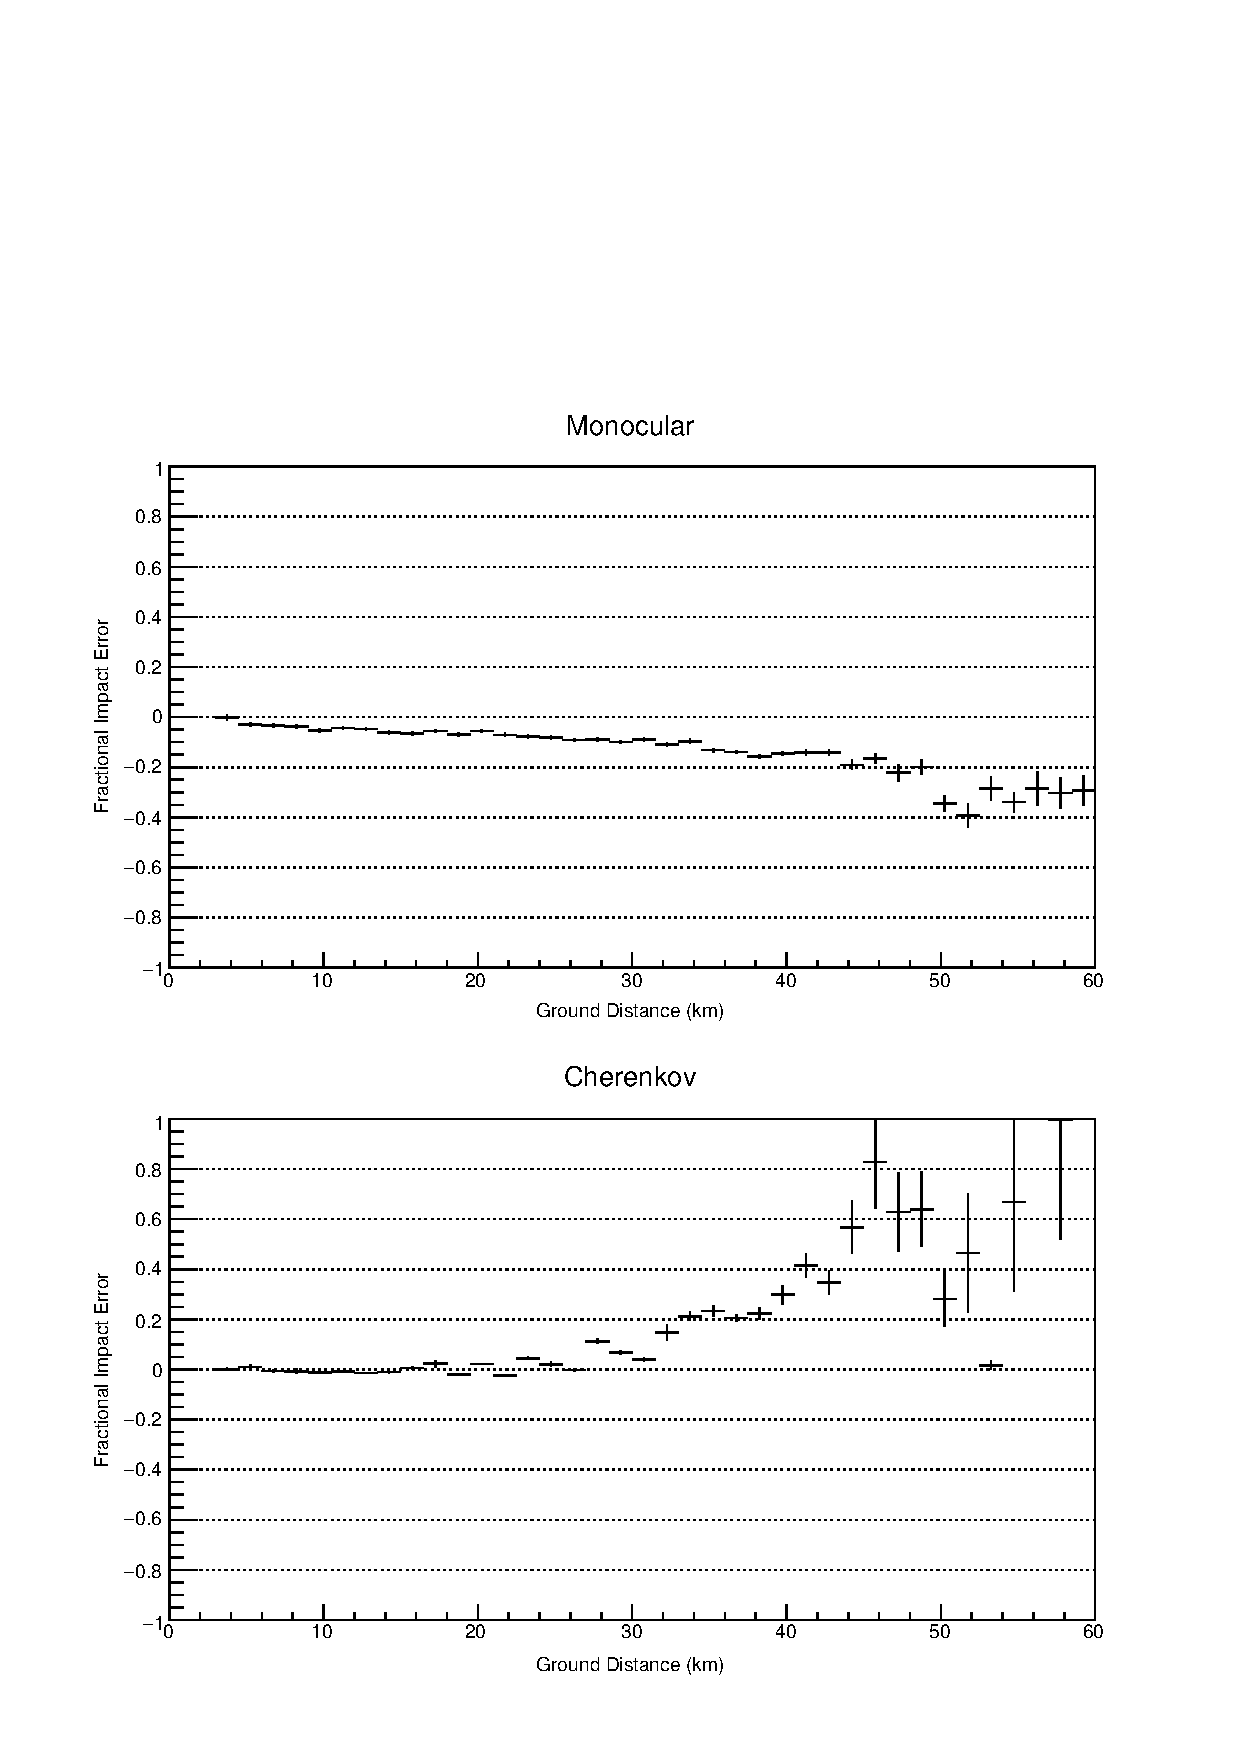
\includegraphics[width=\textwidth]{InitialVersusGround}
    \caption{Results from the initial run with a \SI{200}{m} high detector. Shows the relationship between reconstruction error and ground distance, for both monocular and Cherenkov methods.}
\end{figure}

\begin{figure}[p]
    \label{fig:raised_impact}
    \centering
    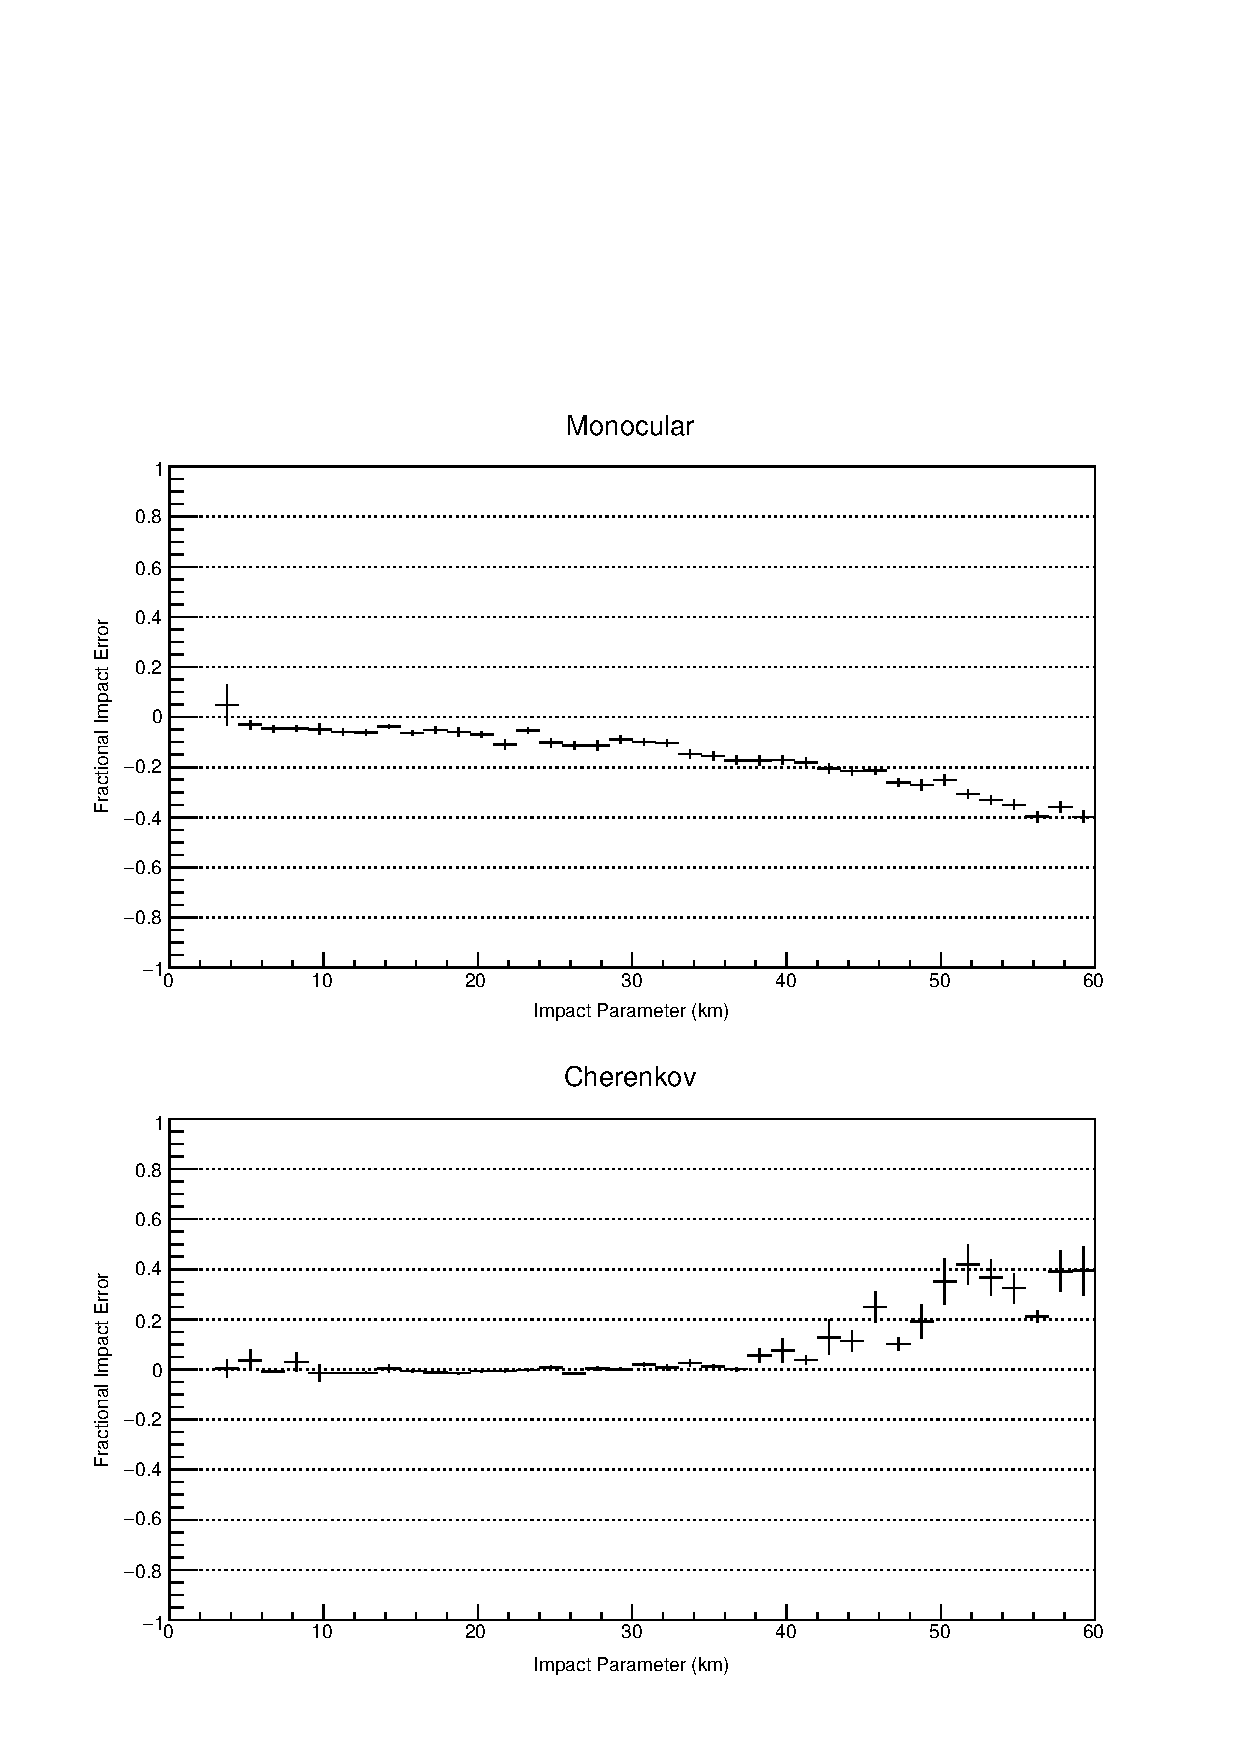
\includegraphics[width=\textwidth]{HighVersusImpact}
    \caption{Results from the second run with a \SI{400}{m} high detector. Shows the relationship between reconstruction error and impact parameter, for both monocular and Cherenkov methods. Note the increased x range of the plot as compared to Figure \ref{fig:error_vs_impact}.}
\end{figure}

\begin{figure}[p]
    \label{fig:raised_gnd}
    \centering
    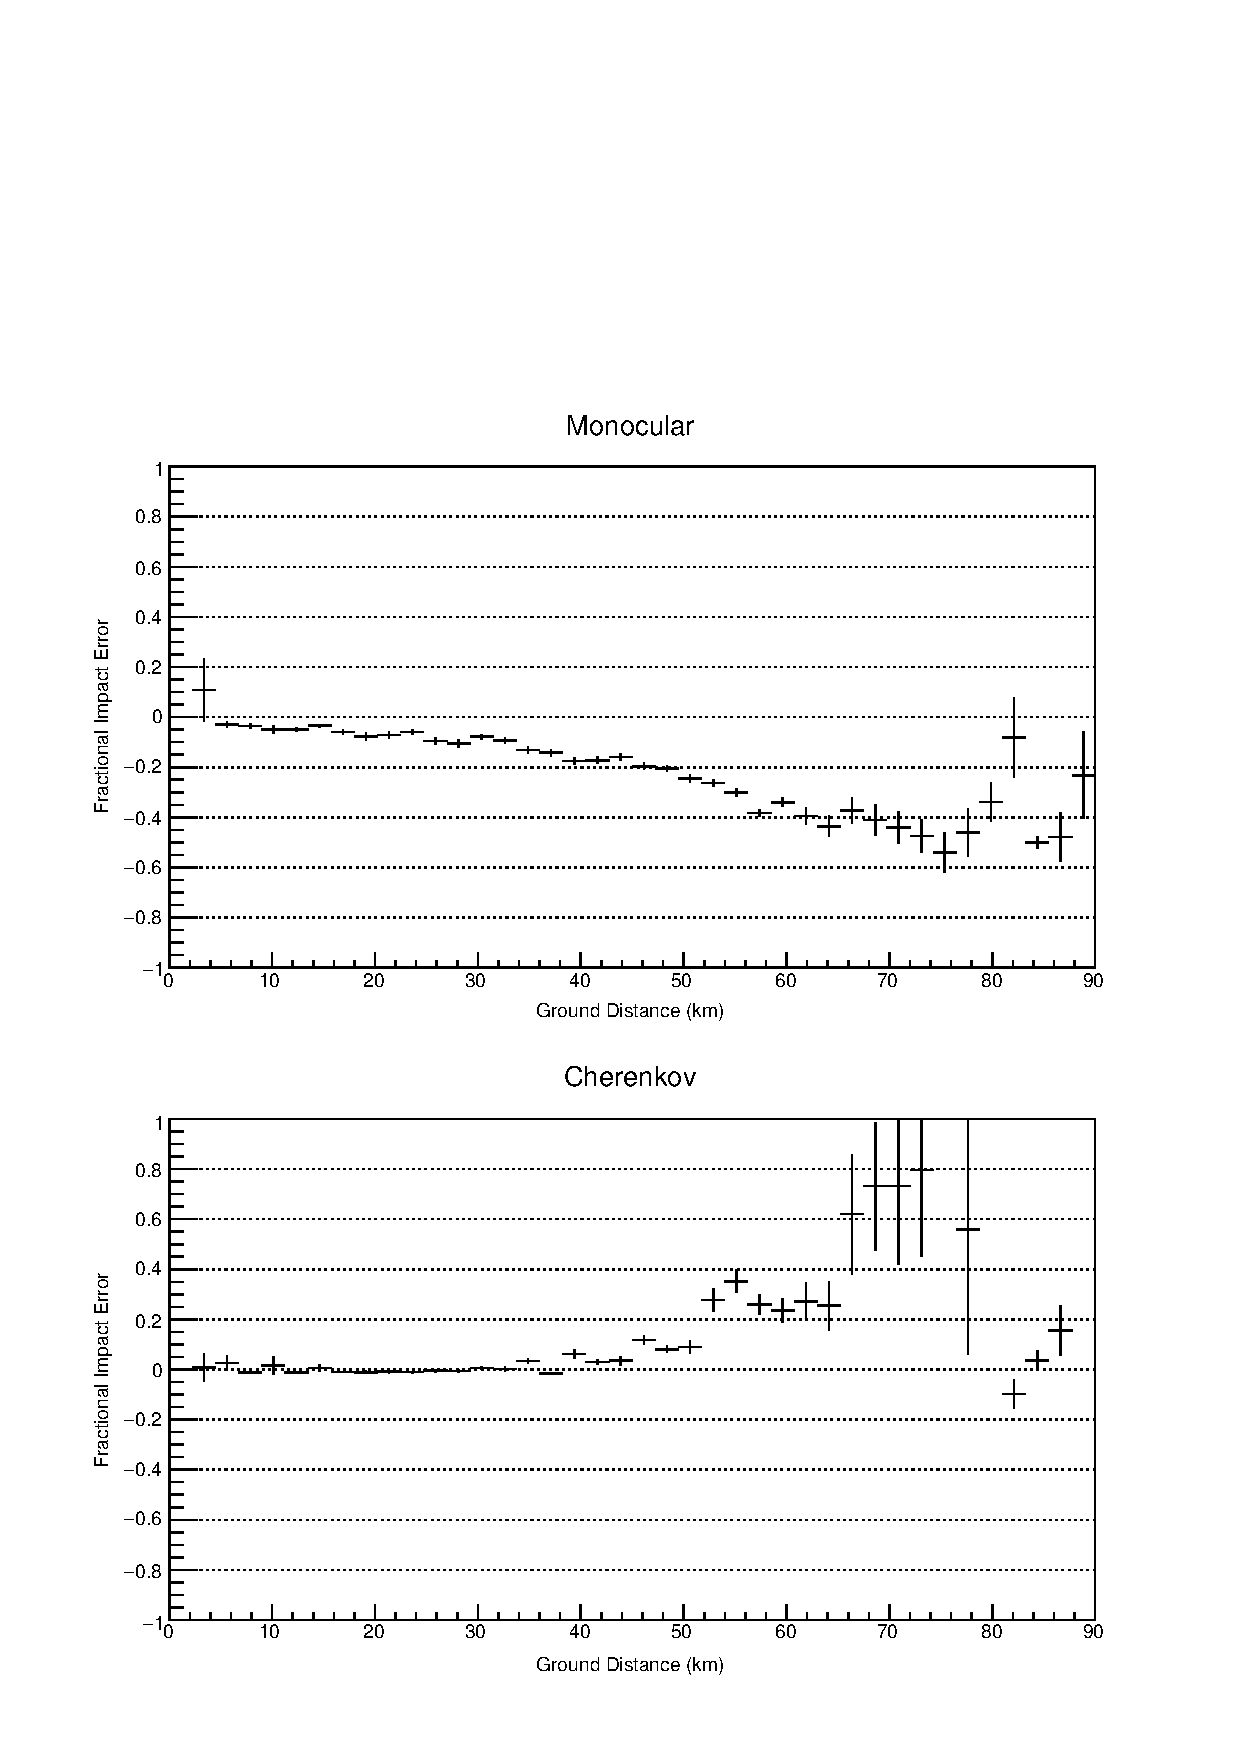
\includegraphics[width=\textwidth]{HighVersusGround}
    \caption{Results from the second run with a \SI{400}{m} high detector. Shows the relationship between reconstruction error and ground distance, for both monocular and Cherenkov methods. Note the increased x range of the plot as compared to Figure \ref{fig:error_vs_gnd}.}
\end{figure}

Based on the results of the \SI{200}{m} simulation, the limits of the Cherenkov reconstruction are set to $\psi > \ang{90}$ or $R_p < \SI{20}{km}$. These bounds are only valid within the subset of the parameter space simulated by the Monte Carlo. Figure \ref{fig:cutoff_hist} compares the overall performance of the two methods under these cuts. Note that there are \num{5573} Cherenkov-reconstructed showers matching the criteria, meaning that the Cherenkov method gives an improvement for about 45 percent of triggered showers. Integrating a Gaussian defined by the parameters in Figure \ref{fig:cutoff_hist} gives an approximation of the expected absolute errors. Under the cuts, the monocular method has an average absolute error of 15.6 percent, while the Cherenkov method has an average absolute error of 10.7 percent. An increase in below-horizon resolution could improve the Cherenkov reconstruction, although it would be unlikely to alter the cuts.

\begin{figure}[p]
    \label{fig:cutoff_hist}
    \centering
    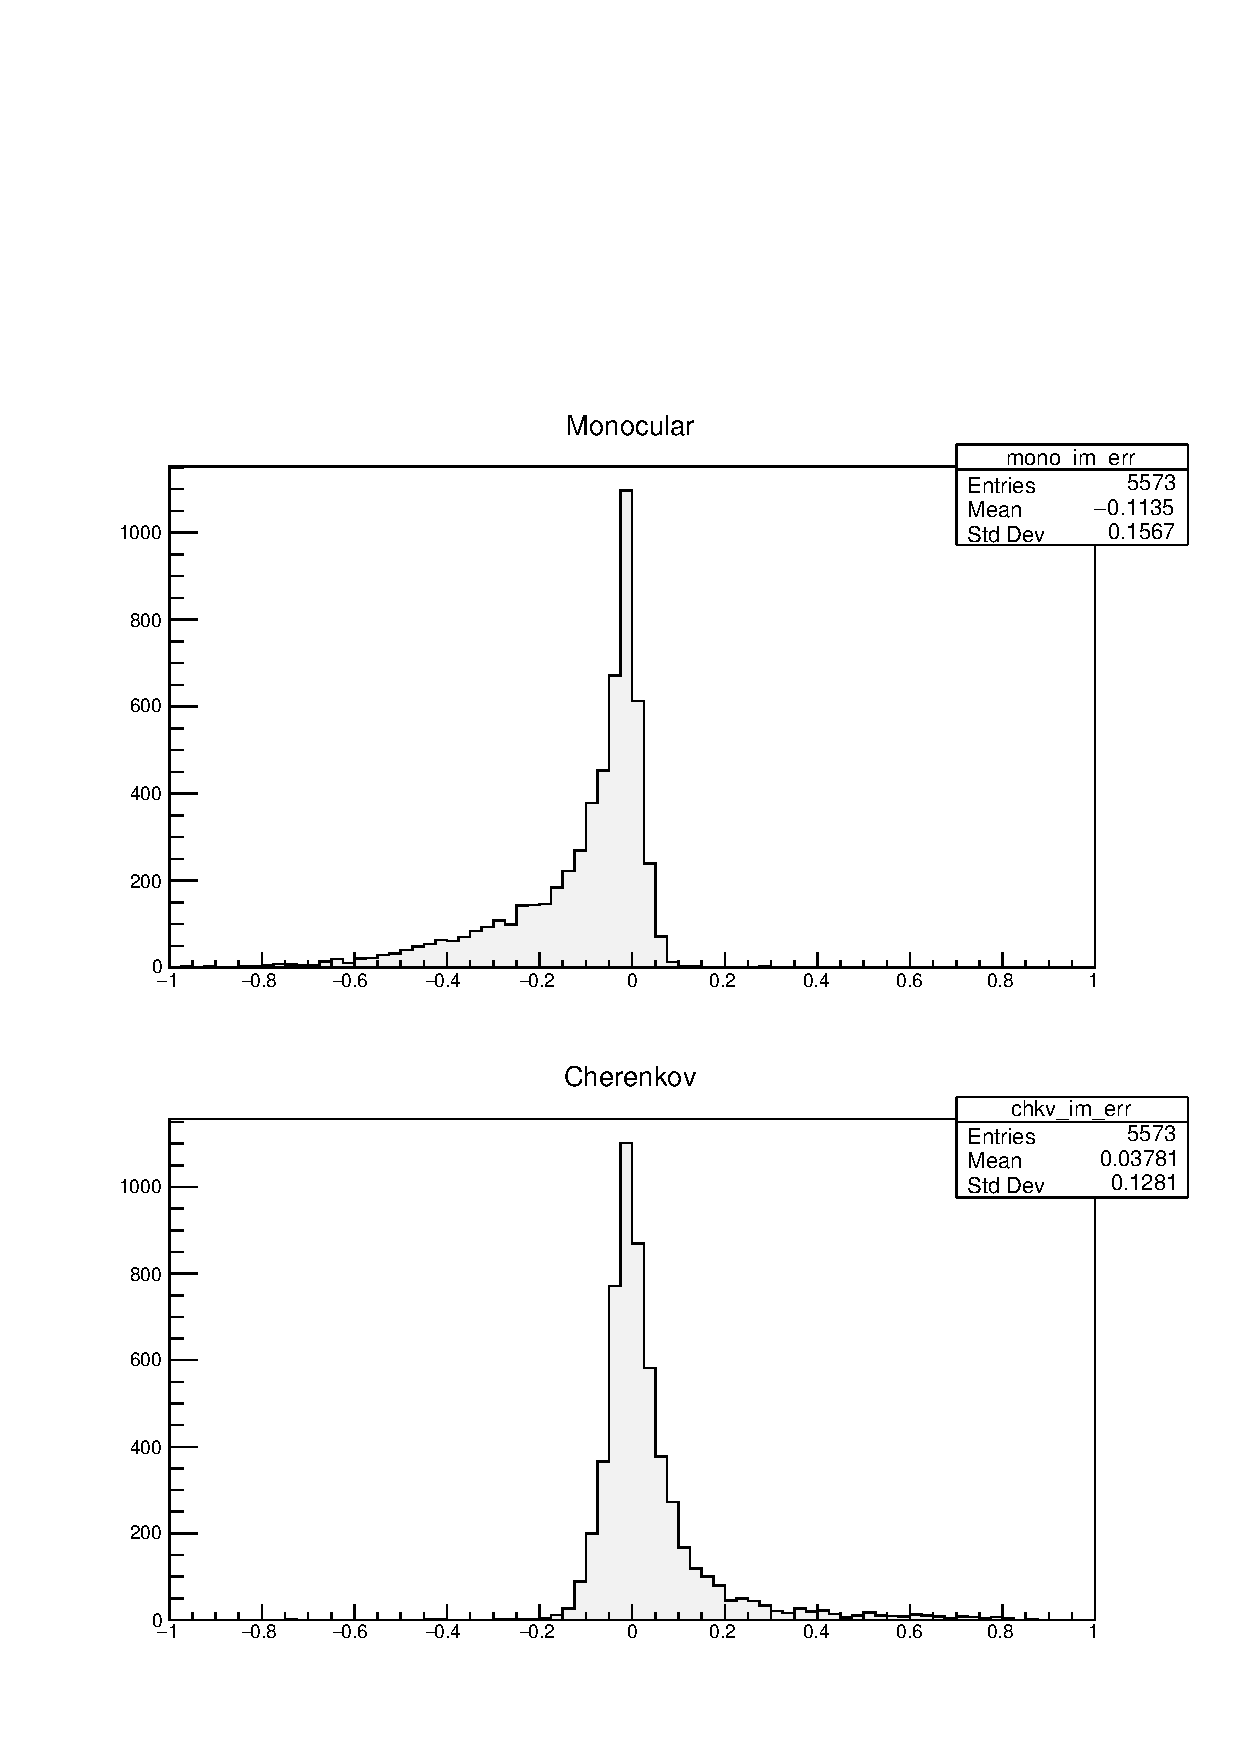
\includegraphics[width=\textwidth]{FinalErrors}
    \caption{The distribution of impact parameter errors from the initial run with a \SI{200}{m} high detector. Cuts of $\psi > \ang{90}$ or $R_p < \SI{20}{km}$ have been applied for the best Cherenkov reconstruction conditions.}
\end{figure}